\documentclass{standalone}

\usepackage{tikz}
\usetikzlibrary{shapes}
\begin{document}


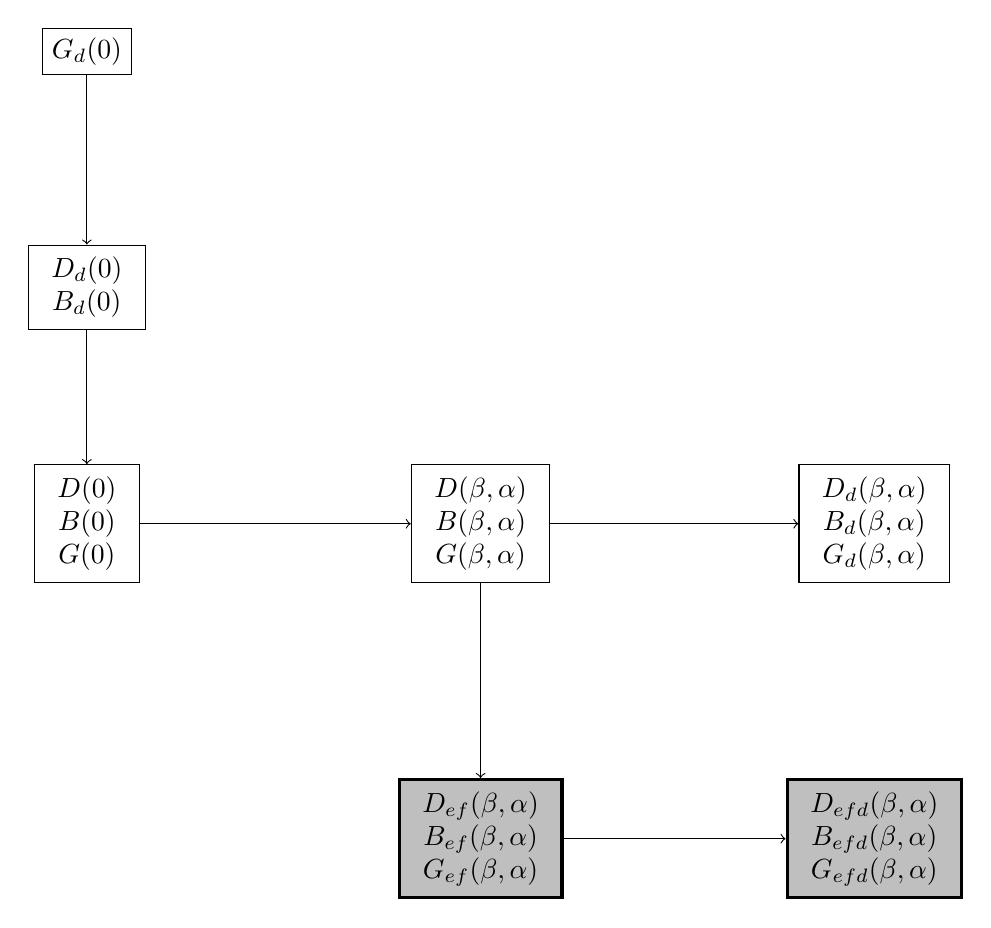
\begin{tikzpicture}
  \node[draw](Gd) at (0,8) {$G_{d}(0)$};
  \node[draw](Dd) at (0,5) {$
      \begin{array}{c}
        D_{d}(0) \\
        B_{d}(0) \\
      \end{array}$};
  \node[draw](G) at (0,2) {$
    \begin{array}{c}
      D(0) \\
      B(0) \\
      G(0)
    \end{array}$};
  \node[draw](Inclin) at (5,2) {$
    \begin{array}{c}
      D(\beta,\alpha) \\
      B(\beta,\alpha) \\
      G(\beta,\alpha)\\
    \end{array}$};
  \node[draw](Inclind) at (10,2) {$
    \begin{array}{c}
      D_{d}(\beta,\alpha) \\
      B_{d}(\beta,\alpha) \\
      G_{d}(\beta,\alpha)
    \end{array}$};
  \node[draw,very thick, fill=lightgray](Eff) at (5,-2){$
    \begin{array}{c}
      D_{ef}(\beta,\alpha) \\ B_{ef}(\beta,\alpha) \\
      G_{ef}(\beta,\alpha)
    \end{array}$};
  \node[draw,very thick, fill=lightgray](Effd) at (10,-2){$
    \begin{array}{c}
      D_{efd}(\beta,\alpha) \\
      B_{efd}(\beta,\alpha) \\
      G_{efd}(\beta,\alpha)
    \end{array}$};

  \draw[->] (Gd) -- (Dd);
  \draw[->] (Dd) -- (G);
  \draw[->] (G) -- (Inclin);
  \draw[->] (Inclin) -- (Inclind);
  \draw[->] (Inclin) -- (Eff);
  \draw[->] (Eff) -- (Effd);
\end{tikzpicture}

\end{document}